\documentclass[withoutpreface,bwprint]{thesis}

\usepackage{fancyhdr}
\usepackage{lastpage}
\usepackage{blindtext}
\usepackage{makecell}
\usepackage[most]{tcolorbox}
\usepackage{minted}
\usepackage{indentfirst}
\lhead{Titanix}

\linespread{1.5}

% \setcounter{tocdepth}{4}

\begin{document}

\thispagestyle{empty}

\begin{figure}[hbt]
    \centering
    
\includegraphics[width=\linewidth]{figure/hitsz_logo.jpg}
\end{figure}

\begin{center}
    \zihao{0}{
        \heiti{Titanix 操作系统}

        \heiti{设计文档}
    }

    \end{center}

    \vspace{3cm}
    \newcommand{\zihaothreetext}[1]{\text{\zihao{3}{#1}}}
    \begin{alignat*}{2}
        & \zihaothreetext{参赛队名:} && \zihaothreetext{Titanix} \\
        & \zihaothreetext{队伍成员:} && \zihaothreetext{曾培鑫、陈佳豪、任秦江} \\
        & \zihaothreetext{指导老师:} && \zihaothreetext{夏文、仇洁婷} \\
    \end{alignat*}
    
    \begin{center}
    \vspace{4cm}
    \zihao{4}{
        全国大学生计算机系统能力大赛 \\
        操作系统赛 \\
        内核实现赛道 \\
        2023年05月 \\
    }
\end{center}

\newpage

\thispagestyle{empty}

\begin{abstract}
    Titanix(Titanic-nix)是一个使用Rust编写的基于Risc-V架构的类Unix操作系统,以异步无栈协程架构为基础,支持多核多任务。目前初赛的所有测试用例已经满分通过,下图是我们队伍(Titanix)的初赛测试通过情况:
\begin{figure}[hbt]
    \centering
    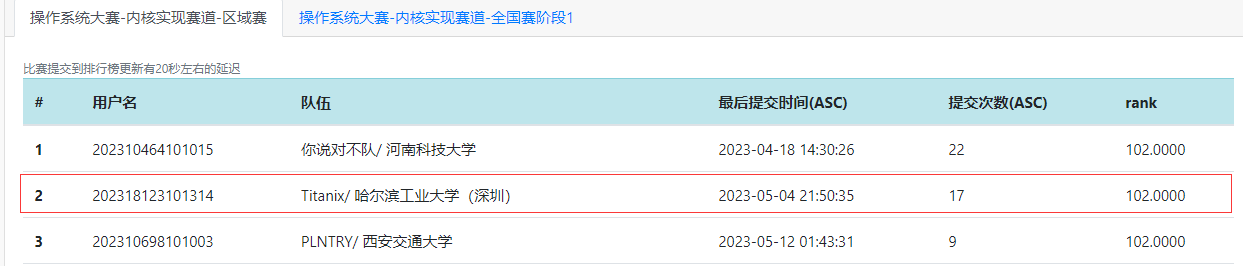
\includegraphics[width=\linewidth]{figure/pre_rank.png}
\end{figure}

此外,Titanix能支持部分libc测试用例以及busybox的部分功能,如sh、ls、echo等,以下是我们各模块的完成情况:

\begin{table}[hbt]
    \caption{Titanix的模块完成情况}
    \centering
    \setlength{\tabcolsep}{10mm}{
    \begin{tabular}{ll}
        \toprule[1.5pt]
        模块 & 完成情况 \\
        \midrule[1pt]
            进程管理   & \makecell[l]{实现分时多任务无栈异步协程调度;\\ 实现多线程运行与回收; \\ 实现多核并行; }      \\
        \midrule[1pt]
            内存管理   & \makecell[l]{实现虚拟内存,用户和内核共享地址空间;\\ 实现页缓存和块缓存,减少IO次数; \\ 实现文件映射和匿名映射;\\ 实现懒分配与写时复制; }     \\
        \midrule[1pt]
            文件系统   & \makecell[l]{实现虚拟文件系统,支持FAT32文件系统接入; \\ 实现Inode缓存,减少IO次数; \\ 利用hash加速Inode查找; \\ TODO}     \\
        \midrule[1pt]
            信号系统   & TODO     \\
        \midrule[1pt]
            多核支持   & TODO     \\
        \bottomrule[1.5pt]
    \end{tabular}
    }
\end{table}


\end{abstract}

\pagestyle{fancy}
% Uncomment the next line to generate a Table of Contents
\setcounter{page}{1}
%%%%%%%%%%%%%%%%%%%%%%%%%%%%%%
%目录
\tableofcontents
\newpage

% main content
\section{概述}

\subsection{完成情况}

\subsection{Titanix 介绍}

\subsection{操作系统整体架构}

\begin{figure}[hbt]
    \centering
    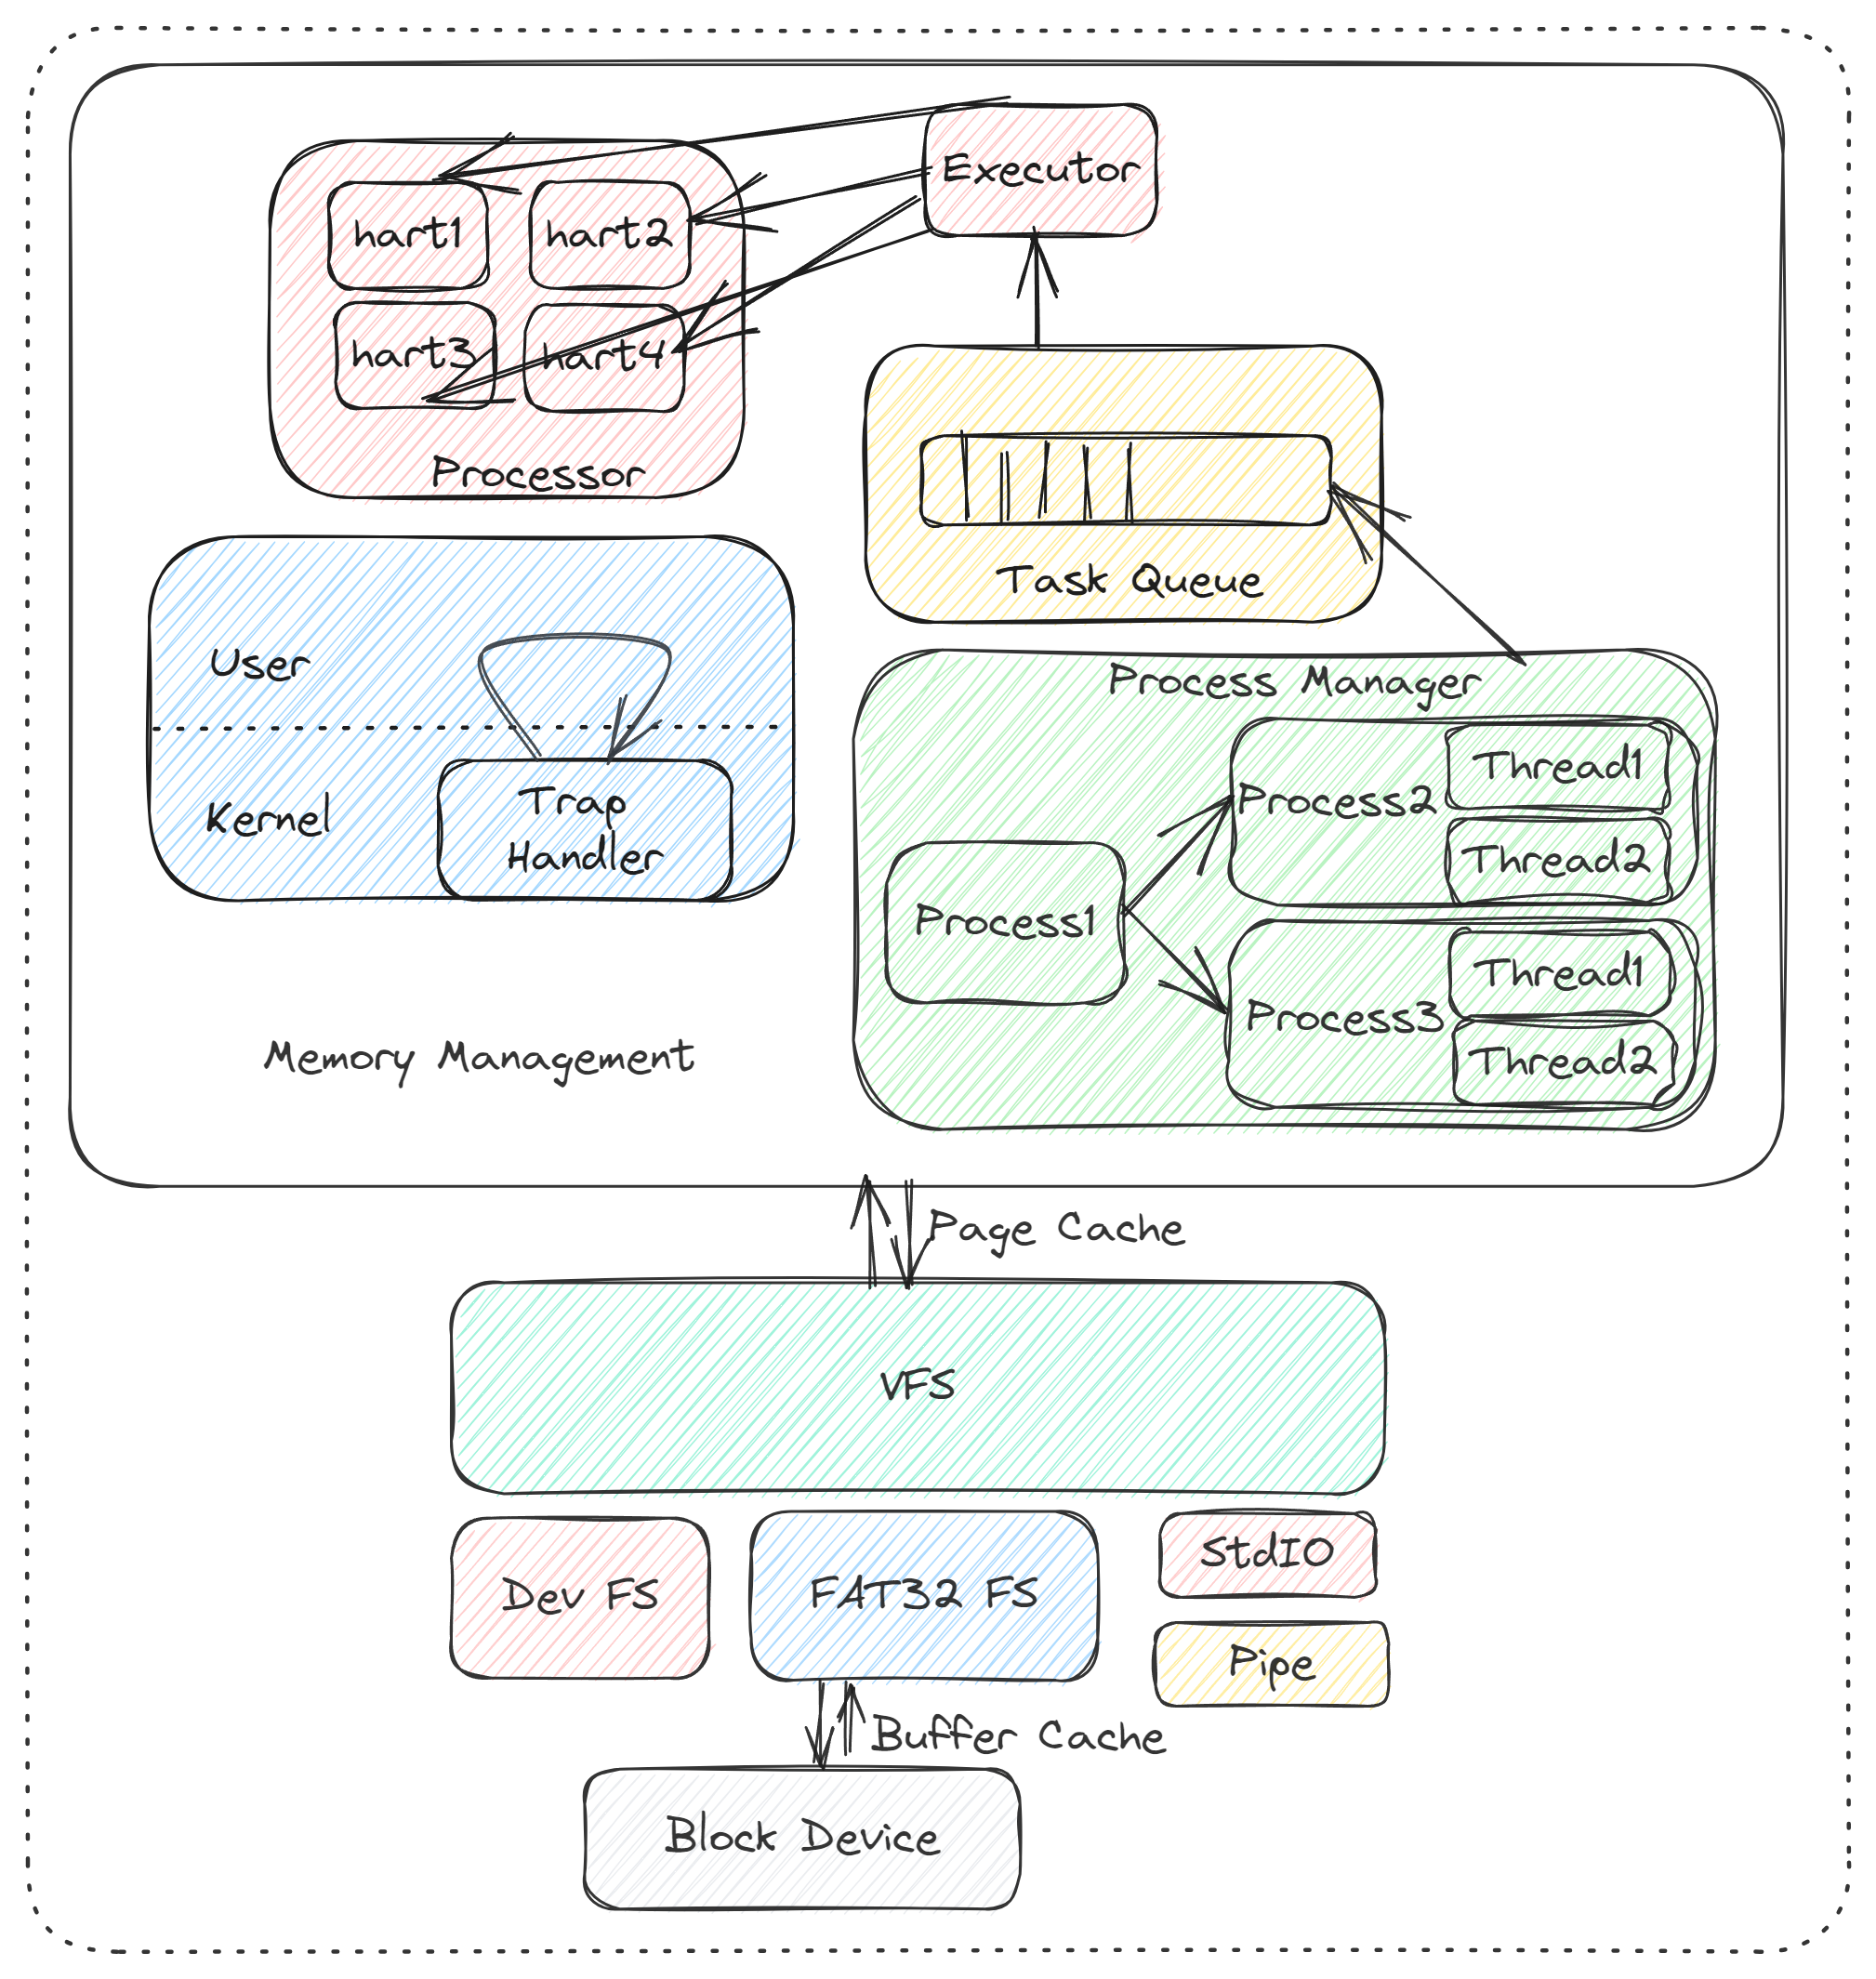
\includegraphics[width=.9\linewidth]{figure/architecture.png}
    \caption{总体架构}
    \label{pic:architecture}
\end{figure}

\subsection{目录和文件描述}

\begin{tcolorbox}[
title=\textbf{os目录树},
listing only,
breakable
]
\begin{minted}[breaklines, baselinestretch=1, fontsize=\small]{text}
|   build.rs
|   gdbinit
|   Makefile
|   tmp.sh
\---src
    |   console.rs
    |   entry.S
    |   lang_items.rs
    |   linker64.ld
    |   loader.rs
    |   main.rs
    |   sbi.rs
    |   timer.rs
    +---boards
    |       mod.rs
    |       qemu.rs
    +---config
    |       board.rs
    |       fs.rs
    |       mm.rs
    |       mod.rs
    |       process.rs
    |       processor.rs
    |       signal.rs
    +---driver
    |   |   mod.rs
    |   \---block
    |           buffer_cache.rs
    |           io_device.rs
    |           mod.rs
    |           sdcard.rs
    |           spi.rs
    |           virtio_blk.rs
    +---executor
    |       mod.rs
    +---fs
    |   |   dirent.rs
    |   |   fd_table.rs
    |   |   file.rs
    |   |   file_system.rs
    |   |   hash_name.rs
    |   |   inode.rs
    |   |   inode_tmp.rs
    |   |   kstat.rs
    |   |   mod.rs
    |   |   pipe.rs
    |   |   stdio.rs
    |   |   uio.rs
    |   |   utsname.rs
    |   +---devfs
    |   |       block_device.rs
    |   |       mod.rs
    |   |       null.rs
    |   |       zero.rs
    |   +---fat32
    |   |       mod.rs
    |   +---fat32_tmp
    |   |       mod.rs
    |   +---procfs
    |   |       mod.rs
    |   \---testfs
    |           mod.rs
    +---mm
    |   |   address.rs
    |   |   frame_allocator.rs
    |   |   heap_allocator.rs
    |   |   mod.rs
    |   |   page.rs
    |   |   page_cache.rs
    |   |   page_table.rs
    |   |   radix_tree.rs
    |   |   recycle_allocator.rs
    |   +---memory_set
    |   |       mod.rs
    |   |       page_fault_handler.rs
    |   |       vm_area.rs
    |   \---user_check
    |           check.S
    |           mod.rs
    +---process
    |   |   manager.rs
    |   |   mod.rs
    |   |   pid.rs
    |   |   _aux.rs
    |   \---thread
    |           exit.rs
    |           mod.rs
    |           schedule.rs
    |           threadloop.rs
    |           thread_resource.rs
    |           thread_state.rs
    |           tid.rs
    +---processor
    |       context.rs
    |       env.rs
    |       hart.rs
    |       mod.rs
    +---signal
    |       mod.rs
    |       signal_context.rs
    |       signal_handler.rs
    +---sync
    |   |   cond_var.rs
    |   |   mod.rs
    |   |   
    |   \---mutex
    |           mod.rs
    |           sleep_mutex.rs
    |           spin_mutex.rs
    +---syscall
    |       dev.rs
    |       fs.rs
    |       mm.rs
    |       mod.rs
    |       process.rs
    |       signal.rs
    |       sync.rs
    +---trap
    |       context.rs
    |       mod.rs
    |       trap.S
    \---utils
        |   error.rs
        |   hash_table.rs
        |   logging.rs
        |   mem.rs
        |   mod.rs
        |   path.rs
        |   string.rs
        \---debug
                mod.rs
                stack_tracker.rs
\end{minted}
\end{tcolorbox}

\subsection{文档相关}

TODO
\section{系统设计与实现}

\subsection{进程管理}

\subsubsection{概述}
进程是操作系统中资源管理的基本单位,而线程是操作系统中调度的基本单位。在linux内核代码里,进程和线程都统一用task\_struct结构体表示。不同于linux内核,Titanix中将进程和线程分别用Process和Thread结构体表示,这样能更加清晰的处理同一进程内不同线程的创建与回收等过程。同一进程的不同线程共享地址空间(包括内核栈),后文会提到,Titanix采用无栈协程的调度方式,所有线程(包括不同进程的线程)共享同一个内核栈,调度起来开销比较小。

\subsubsection{进程控制块}

\begin{tcolorbox}[title=\textbf{os/src/process/mod.rs}]
\begin{minted}[baselinestretch=1, fontsize=\small]{rust}
/// Process control block
pub struct Process {
    /// immutable
    pid: PidHandle,
    /// mutable
    inner: SpinNoIrqLock<ProcessInner>,
}
\end{minted}
\end{tcolorbox}

我们将进程控制块分为可变和不可变的两个部分,后文会提到,进程控制块的所有权由其父进程和其包含的所有线程持有,在Rust中,对于这种有多个所有权的情况,我们需要用一个Arc(Atomic reference count)将其包裹,而Arc在Rust中默认是不可变的,因此对于可变部分,我们需要用互斥锁将其包裹;由于进程一创建便会分配一个进程ID且在其生命周期内不可变,因此我们将其归为不可变部分,对于可变部分,具体成员如下:
\begin{tcolorbox}[
title=\textbf{os/src/process/mod.rs},
listing only,
breakable
]
\begin{minted}[baselinestretch=1, fontsize=\small]{rust}
/// Process control block inner
pub struct ProcessInner {
    /// Whether this process is a zombie process
    pub is_zombie: bool,
    /// The process's address space
    pub memory_set: MemorySet,
    /// Parent process
    pub parent: Option<Weak<Process>>,
    /// Children processes
    pub children: Vec<Arc<Process>>,
    /// File descriptor table
    pub fd_table: FdTable,
    /// Allocate tid
    pub tid_allocator: RecycleAllocator,
    /// TODO: use BTreeMap to query and delete more quickly
    pub threads: Vec<Weak<Thread>>,
    /// Signal handlers for every signal
    pub sig_handler: Arc<SpinNoIrqLock<SigHandlerManager>>,
    /// Pending sigs that wait for the prcoess to handle
    pub pending_sigs: SigQueue,
    /// UStack base of all threads(the lowest bound)
    pub ustack_base: usize,
    /// Addr -> Condvar map
    pub addr_to_condvar_map: BTreeMap<usize, CondVar>,
    /// Exit code of the current process
    /// Note that we may need to put this member in every thread
    pub exit_code: i8,
    /// Current Work Directory
    /// Maybe change to Dentry later.
    pub cwd: String,
}
\end{minted}
\end{tcolorbox}
每个成员的作用如注释所述,值得注意的是,进程对所有孩子进程持有强引用(即所有权),而对父进程持有弱引用(没有所有权),这样做能防止循环引用导致内存泄漏;另外进程对其所有的线程也是持弱引用,因为某个线程可以在进程还未退出时先退出并释放内存。

\subsubsection{线程控制块}
\begin{tcolorbox}[title=\textbf{os/src/process/thread/mod.rs}]
\begin{minted}[baselinestretch=1, fontsize=\small]{rust}
/// Thread control block
pub struct Thread {
    /// immutable
    pub tid: TidHandle,
    /// the process this thread belongs to
    pub process: Arc<Process>,
    // /// whether the user specify the stack
    // pub user_specified_stack: bool,
    /// mutable
    pub inner: UnsafeCell<ThreadInner>,
}
\end{minted}
\end{tcolorbox}
类似进程控制块,我们也将线程控制块分成可变和不可变部分,不可变部分包括线程ID和该线程所属进程的Arc指针,对于可变部分,我们采用了UnsafeCell而不是像进程控制块一样采用SpinNoIrqLock,原因是UnsafeCell可以不需要加锁从而修改内部成员,顾名思义,这一行为在编译器看来是不安全的,不安全是因为编译器无法帮我们保证不同线程对该结构体的互斥访问,但对于我们的内核来说,这个成员只会在当前核心进行访问,即不可能出现在某一线程里访问另一线程的这个成员,对于这个成员,其拥有的具体子成员如下:
\begin{tcolorbox}[title=\textbf{os/src/process/thread/mod.rs}]
\begin{minted}[baselinestretch=1, fontsize=\small]{rust}
/// Thread inner,
/// This struct can only be visited by the local hart except the `terminated` field
/// which is the reason why it is an atomic variable
pub struct ThreadInner {
    // TODO: add more members
    /// Trap context that saves both kernel and user msg
    pub trap_context: TrapContext,
    /// Used for signal handle
    pub signal_context: Option<SignalContext>,
    /// When invoking `exec`, we need to get the ustack base.
    /// Note that ustack_base is the base of all ustacks
    pub ustack_base: usize,
    /// Thread state.
    /// Note that this may be modified by another thread, which
    /// need to be sync
    pub state: ThreadStateAtomic,
    /// Tid address, which may be modified by `set_tid_address` syscall
    pub tid_addr: Option<TidAddress>,
}
\end{minted}
\end{tcolorbox}
每个成员的具体作用如注释所述,值得注意的是,我们可能会出现在主线程里强制杀死别的子线程的情况,这个时候可能需要跨线程访问ThreadInner结构体并修改其state成员,因此我们将其设为原子变量,防止并发问题。

\subsubsection{线程调度}\label{schedule}

本系统的线程调度模型采用的是无栈异步协程架构, 协程即协作式多任务的子例程,协作式指的是协程的调度(挂起或运行)是由协程本身决定而不是被抢占式的;为什么说线程调度模型是协程架构呢?从用户态来说线程显然不符合协作式的概念(需要被内核抢占式调度),但从内核态来看,内核拥有线程的所有权,可以自行决定在某个时候将某个线程挂起或切换(如时钟中断的到来等),因此可以说OS中的线程对内核态来说便是协程。以下是无栈协程和有栈协程的区别:

\paragraph{有栈协程}~{}

每一个协程(即操作系统的线程)拥有自己独立的栈,每次进行协程的切换时需要修改栈指针,手动保存所有上下文信息如通用寄存器并切换为目标协程的通用寄存器,另外协程切换前后需要考虑是否有互斥锁或其他资源尚未释放,否则容易造成死锁。调度过程如\cref{pic:stack_coroutine}所示。
\begin{figure}[hbt]
    \centering
    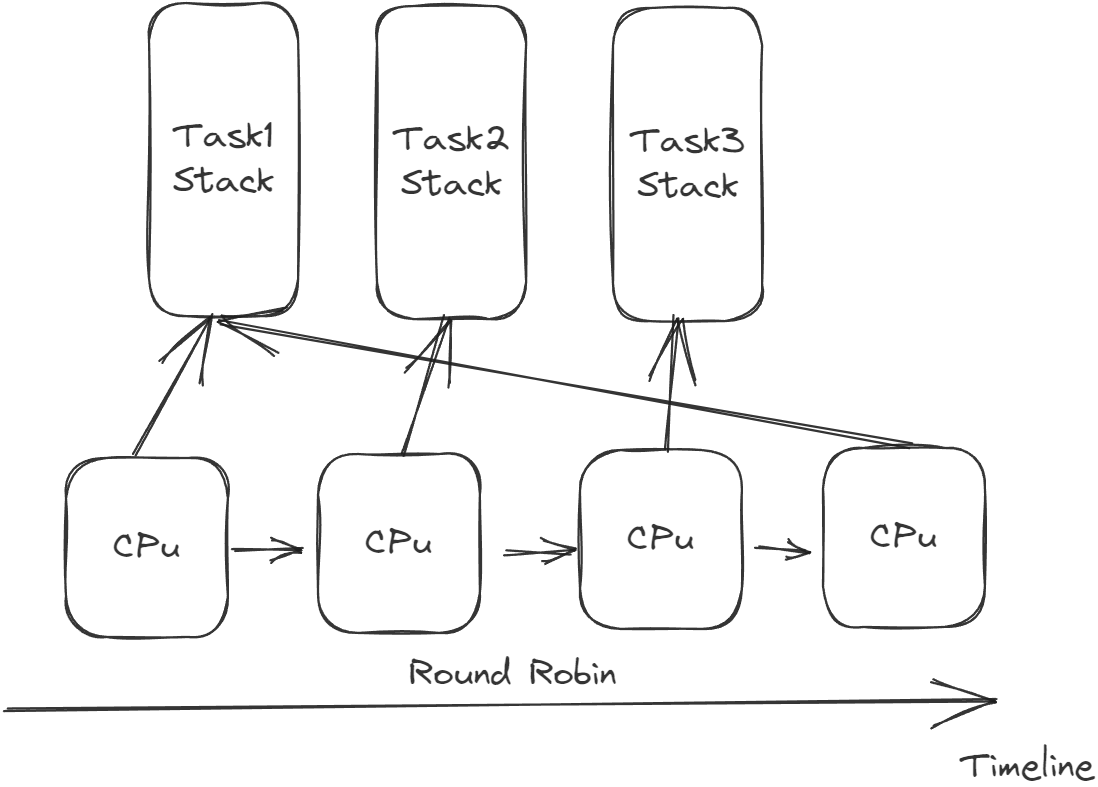
\includegraphics[width=.9\linewidth]{figure/stack_coroutine.png}
    \caption{有栈协程调度}
    \label{pic:stack_coroutine}
\end{figure}

\paragraph{无栈协程}~{}

所有的协程共用一个栈,每个协程在堆上维护一个状态机,协程的切换是通过轮询当前的状态,然后根据状态决定是否需要切换,下述代码为简单示例:

\begin{tcolorbox}[
title=\textbf{coroutine example},
listing only,
breakable
]
    \begin{minted}[baselinestretch=1, fontsize=\small]{rust}
enum PollResult {
    Ready,
    Pending,
}

enum State {
    StateA,
    StateB,
    StateC,
}

struct Coroutine {
    state: State,
}

impl Coroutine {
    pub fn poll(&mut self) -> PollResult {
        match self.state {
            State::StateA => {
                /* Do something */
                self.state = State::StateB;
                return PollResult::Pending;
            }
            State::StateB => {
                /* Do something */
                self.state = State::StateC;
                return PollResult::Pending;
            }
            State::StateC => {
                /* Do something */
                return PollResult::Ready;
            }
        }
    }
}
    \end{minted}
\end{tcolorbox}

上述代码中的poll函数即为协程的具体运行函数,不难看出其是一个状态机模型,上层每次调用poll时都可能改变其状态,从而推进其运行;总的来说,无栈协程的调度是通过函数返回然后调用另一个函数实现的,而不是像有栈协程那样直接原地更改栈指针,如下\cref{pic:nonstack_coroutine}所示。
\begin{figure}[hbt]
    \centering
    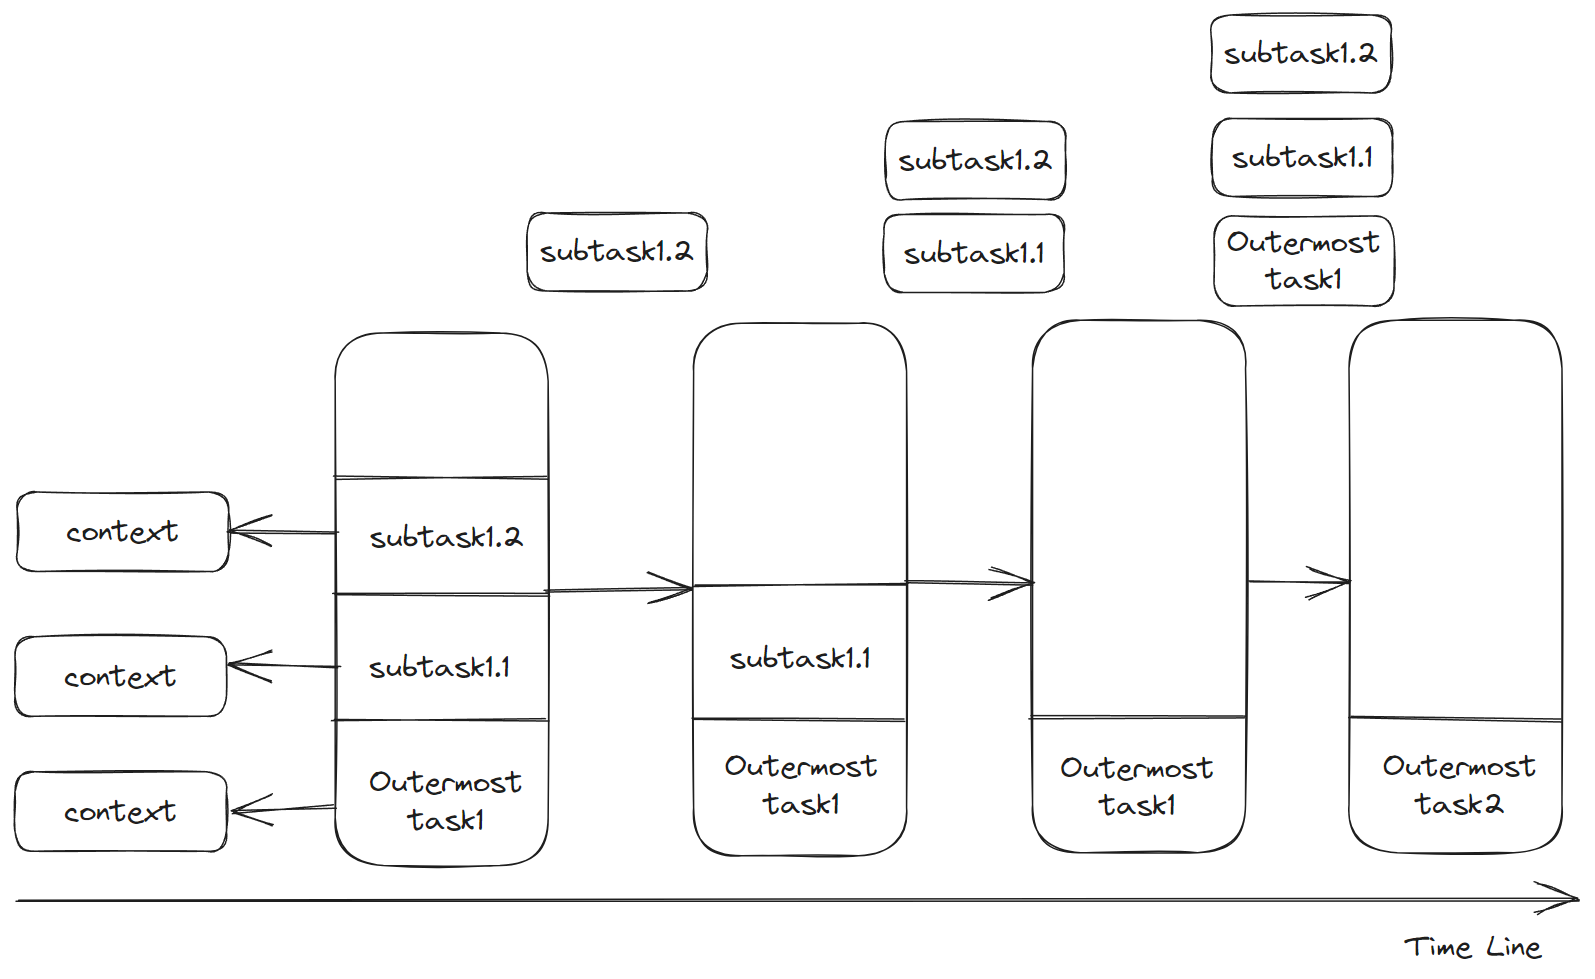
\includegraphics[width=.9\linewidth]{figure/nonstack_coroutine.png}
    \caption{无栈协程调度}
    \label{pic:nonstack_coroutine}
\end{figure}

\paragraph{Rust中的async/await}~{}

在Rust中,将一个函数定义为async或者使用async move {}包裹的代码块即为一个无栈协程,称为一个future。对于一个future,Rust会将其编译成类似上述状态机的形式,然后用户通过.await使其开始运行(即调用poll函数),因此我们可以为每一个线程设置一个future,大致框架如下:

\begin{tcolorbox}[
title=\textbf{os/src/process/thread/schedule.rs},
listing only,
breakable
]
    \begin{minted}[breaklines, baselinestretch=1, fontsize=\small]{rust}
impl<F: Future + Send + 'static> Future for UserTaskFuture<F> {
    type Output = F::Output;
    fn poll(self: Pin<&mut Self>, cx: &mut Context<'_>) -> Poll<Self::Output> {
        let this = unsafe { self.get_unchecked_mut() };
        let hart = processor::local_hart();
        
        hart.push_task(&mut this.task_ctx);
        // run the `threadloop`
        let ret = unsafe { Pin::new_unchecked(&mut this.task_future).poll(cx) };
        hart.pop_task(&mut this.task_ctx);
        
        ret
    }
}
    \end{minted}
\end{tcolorbox}

上述代码中的UserTaskFuture即为每个线程对应的无栈协程运行逻辑,在poll函数中,我们先获得当前核心(在\hyperref[multiharts]{多核心管理}中详细介绍),做一些运行新线程的准备工作(如切换页表等),然后便可以开始轮询具体的线程处理函数,每个线程的运行函数实际上是一个死循环,一直运行直至线程退出,其具体逻辑大体如下:
\begin{tcolorbox}[
title=\textbf{os/src/process/thread/threaloop.rs},
listing only,
breakable
]
    \begin{minted}[breaklines, baselinestretch=1, fontsize=\small]{rust}
pub async fn threadloop(thread: Arc<Thread>) {
    loop {
        let trap_context = unsafe {
            let p = &mut *thread.inner.get();
            &mut p.trap_context
        };
        trap::trap_return(trap_context);
        trap::trap_handler().await;
        if thread.is_zombie() {
            break;
        }
    }
    // When the process becomes zombie, all of its threads should exit too
    handle_exit(&thread);
}
    \end{minted}
\end{tcolorbox}

如上代码所示,一个线程的生命周期内做的事情就是不断重复“回到用户态执行用户态代码->由于中断或异常陷入内核进行处理”这个过程。

\paragraph{线程调度}~{}

介绍完上述关于无栈协程和Rust的async/await,我们还需要一个执行器来调度这些协程(future),这里我们采用了第三方库async-task,这个库可以构造一个future执行器来调度内核的所有任务。首先我们需要维护一个全局任务队列,然后执行器依次从全局队列中取出任务执行,只要我们的OS还有线程在跑(至少initproc永不消亡),那任务队列里就始终有任务,具体逻辑如下:
\begin{tcolorbox}[
title=\textbf{os/src/executor/mod.rs},
listing only,
breakable
]
    \begin{minted}[breaklines, baselinestretch=1, fontsize=\small]{rust}
/// Return the number of the tasks executed
pub fn run_until_idle() -> usize {
    let mut n = 0;
    loop {
        if let Some(task) = TASK_QUEUE.fetch_task() {
            // info!("fetch a task");
            task.run();
            n += 1;
        } else {
            break;
        }
    }
    n
}
    \end{minted}
\end{tcolorbox}

\paragraph{线程唤醒}~{}

Rust中的future在轮询的过程中会传入一个waker句柄,可以通过其来唤醒上层任务,我们的内核线程可以通过该句柄将某个线程唤醒,并且重新加入任务队列;

总体来看,线程调度是一个Round-Robin的过程,内核维护一个固定的时间片,每次时间片一到,会产生一个时钟中断,用户线程陷入内核,在trap\_handler函数处await出去,然后上层执行器便从任务队列中取出下一个任务,不断重复此过程即可实现分时多任务。

\subsubsection{异常与中断}
OS内核控制和调度用户程序以及各个外设硬件的方式就是异常和中断。对于RISC-V架构来说,stvec寄存器会存储中断向量,每次有异常或中断发生时,pc寄存器会被设置为stvec中存储的中断向量的值。因此我们需要做的就是实现一个异常或中断处理函数,然后将其地址存入stvec寄存器中。

\paragraph{返回用户态}~{}

返回用户态这一过程大体上来说会在两个地方用到:当一个进程在内核态被构建出来后首先要做的事情就是返回用户态去执行elf文件中的代码,此时要经历该过程;当一个进程因为异常或者中断陷入内核之后,要重新返回用户态,此时要经历该过程。由于Titanix的内核和用户共用页表,我们返回用户态的操作也比较简单。具体来说,可以把返回用户态这一步看成一个正常的函数调用,因此只需要手动保存caller-saved寄存器即可(其他寄存器会在编译的时候自动保存到内核栈中),代码如下所示:
\begin{tcolorbox}[
title=\textbf{os/src/trap/mod.rs},
listing only,
breakable
]
    \begin{minted}[breaklines, baselinestretch=1, fontsize=\small]{rust}
#[no_mangle]
/// Back to user mode.
/// Note that we don't need to flush TLB since user and
/// kernel use the same pagetable.
pub fn trap_return(trap_context: &mut TrapContext) {
    set_user_trap_entry();
    extern "C" {
        // fn __alltraps();
        fn __return_to_user(cx: *mut TrapContext);
    }

    check_signal_for_current_process();
    unsafe {
        __return_to_user(trap_context);
    }
}
    \end{minted}
\end{tcolorbox}

\_\_return\_to\_user是一个汇编函数,所做的事情就是手动保存所有的caller-saved寄存器,然后将用户态的所有通用寄存器(在下一部分 陷入内核 会讲)一并恢复,最后将TrapContext的地址保存在sscratch寄存器中。另外,值得注意的是,当一个进程刚刚被构建出来的时候,我们需要在内核态给他的用户态通用寄存器赋初值,默认是0,但栈指针需要根据我们设定的用户态栈进行赋值。

\paragraph{陷入内核}~{}

在用户因系统调用、时钟中断、缺页中断等原因发生异常和中断时,会跳转stvec中存储的中断向量,我们需要保存用户态的上下文,具体包括32个通用寄存器和sepc寄存器,当返回用户态时保存的通用寄存器可以恢复现场,sepc寄存器可以让用户态在发生异常的指令处或者下一条指令处继续执行。我们要想在中断向量中保存这些寄存器,由于此时已经处于内核态了,我们还需要一个内核结构体来保存,因此在陷入内核时需要知道该内核结构体的地址。RISC-V中有一个特权寄存器sscratch可以用来存放核心相关的上下文的地址,在前文中有提到,我们再返回用户态时会将TrapContext的地址存入sscratch中,因此这个时候便可以用其来保存用户上下文。

\paragraph{陷阱处理函数}~{}

由于我们的内核是异步的,结合了Rust的async/await机制,因此自然要将陷进处理函数(即trap handler)定义为异步函数,实际上,内核的进程切换点也是在trap handler中。

具体来说,我们在trap handler中对不同的中断或异常类型进行相应的处理,对于每种情况,可能的结果有:
\begin{enumerate}
    \item 正常处理并返回用户态;
    \item 发生用户态严重异常,导致进程直接退出,不会再返回用户态;
    \item 时钟中断,当前进程切换到下一个进程(严格来说是线程),此时该进程会一直等到下一次调度到自己后才返回用户态;
\end{enumerate}

\subsubsection{多核心管理}\label{multiharts}
对于RISC-V架构来说,每个核心有自己独立的一套寄存器,因此从总体上看,只需要给每个核心划分好内核栈,便可以开始进行并行调度运行,多核内存管理在下一章节讨论。这里我们重点关注多核运行,前面\hyperref[schedule]{线程调度}中提到,每次取出新的任务时,我们需要拿到当前的核心,而我们将每个核心的核心控制块地址存放在tp寄存器中,因此可以通过读取tp寄存器来获取当前核心,核心控制块的定义如下:
\begin{tcolorbox}[
title=\textbf{os/src/processor/hart.rs},
listing only,
breakable
]
    \begin{minted}[breaklines, baselinestretch=1, fontsize=\small]{rust}
pub struct Hart {
    hart_id: usize,
    /// Spare env ctx when in need(e.g. kernel thread or idle thread)
    spare_env_ctx: EnvContext,
    local_ctx: LocalContext,
    /// Every hart has its own kernel stack
    kstack_bottom: usize,
}
    \end{minted}
\end{tcolorbox}
核心控制块的关键成员在于local\_ctx成员,该成员可以在挂上各种各样的per-CPU的成员,目前有栈追踪器(用来记录调用栈)、页表和线程控制块,线程控制块即当前核心正在运行的线程,每次调度新的任务时需要修改satp值以启用新的页表,同时刷新TLB。
\subsection{内存管理}

\subsubsection{概述}

在Titanix中,内核和用户共享地址空间,因此在陷入内核和返回用户态不需要像rCore-tutorial那样进行繁琐的处理,不需要trampoline页面,只需要正常跳转即可。对于内核的地址空间,我们采用直接映射,对于用户的地址空间,我们采用物理页帧随机映射。

\subsubsection{地址空间}

在QEMU平台上,内核的入口地址是在0x8020\_0000,若将0x8000\_0000以下部分作为用户的地址空间,那用户态便只有2G的地址空间,若是在U740开发板上则无法完全利用其内存,又因为RISC-V SV39的规定,内存地址空间只能分布在0x0至0x3f\_ffff\_ffff和0xffff\_ffc0\_0000\_0000至0xffff\_ffff\_ffff\_ffff,因此我们将用户地址空间映射到0x0至0x3f\_ffff\_ffff,内核地址空间映射到0xffff\_ffc0\_0000\_0000至0xffff\_ffff\_ffff\_ffff。\\

\paragraph{内核地址空间}~{}

内核地址空间见下\cref{pic:kernel_mem}所示,可以看到内核的入口地址位于0xffff\_ffc0\_8020\_0000,我们首先在链接脚本中将链接基址改为0x8020\_0000,由于生成的内核elf文件不是位置无关代码(或许可以通过编译选项设置为PIC?),而QEMU默认跳转到的内核第一条指令为0x8020\_0000,因此我们需要在内核启动的时候就尽快将地址空间映射到高位,否则可能会因为跳转绝对地址导致内核崩溃。
\begin{figure}[hbt]
    \centering
    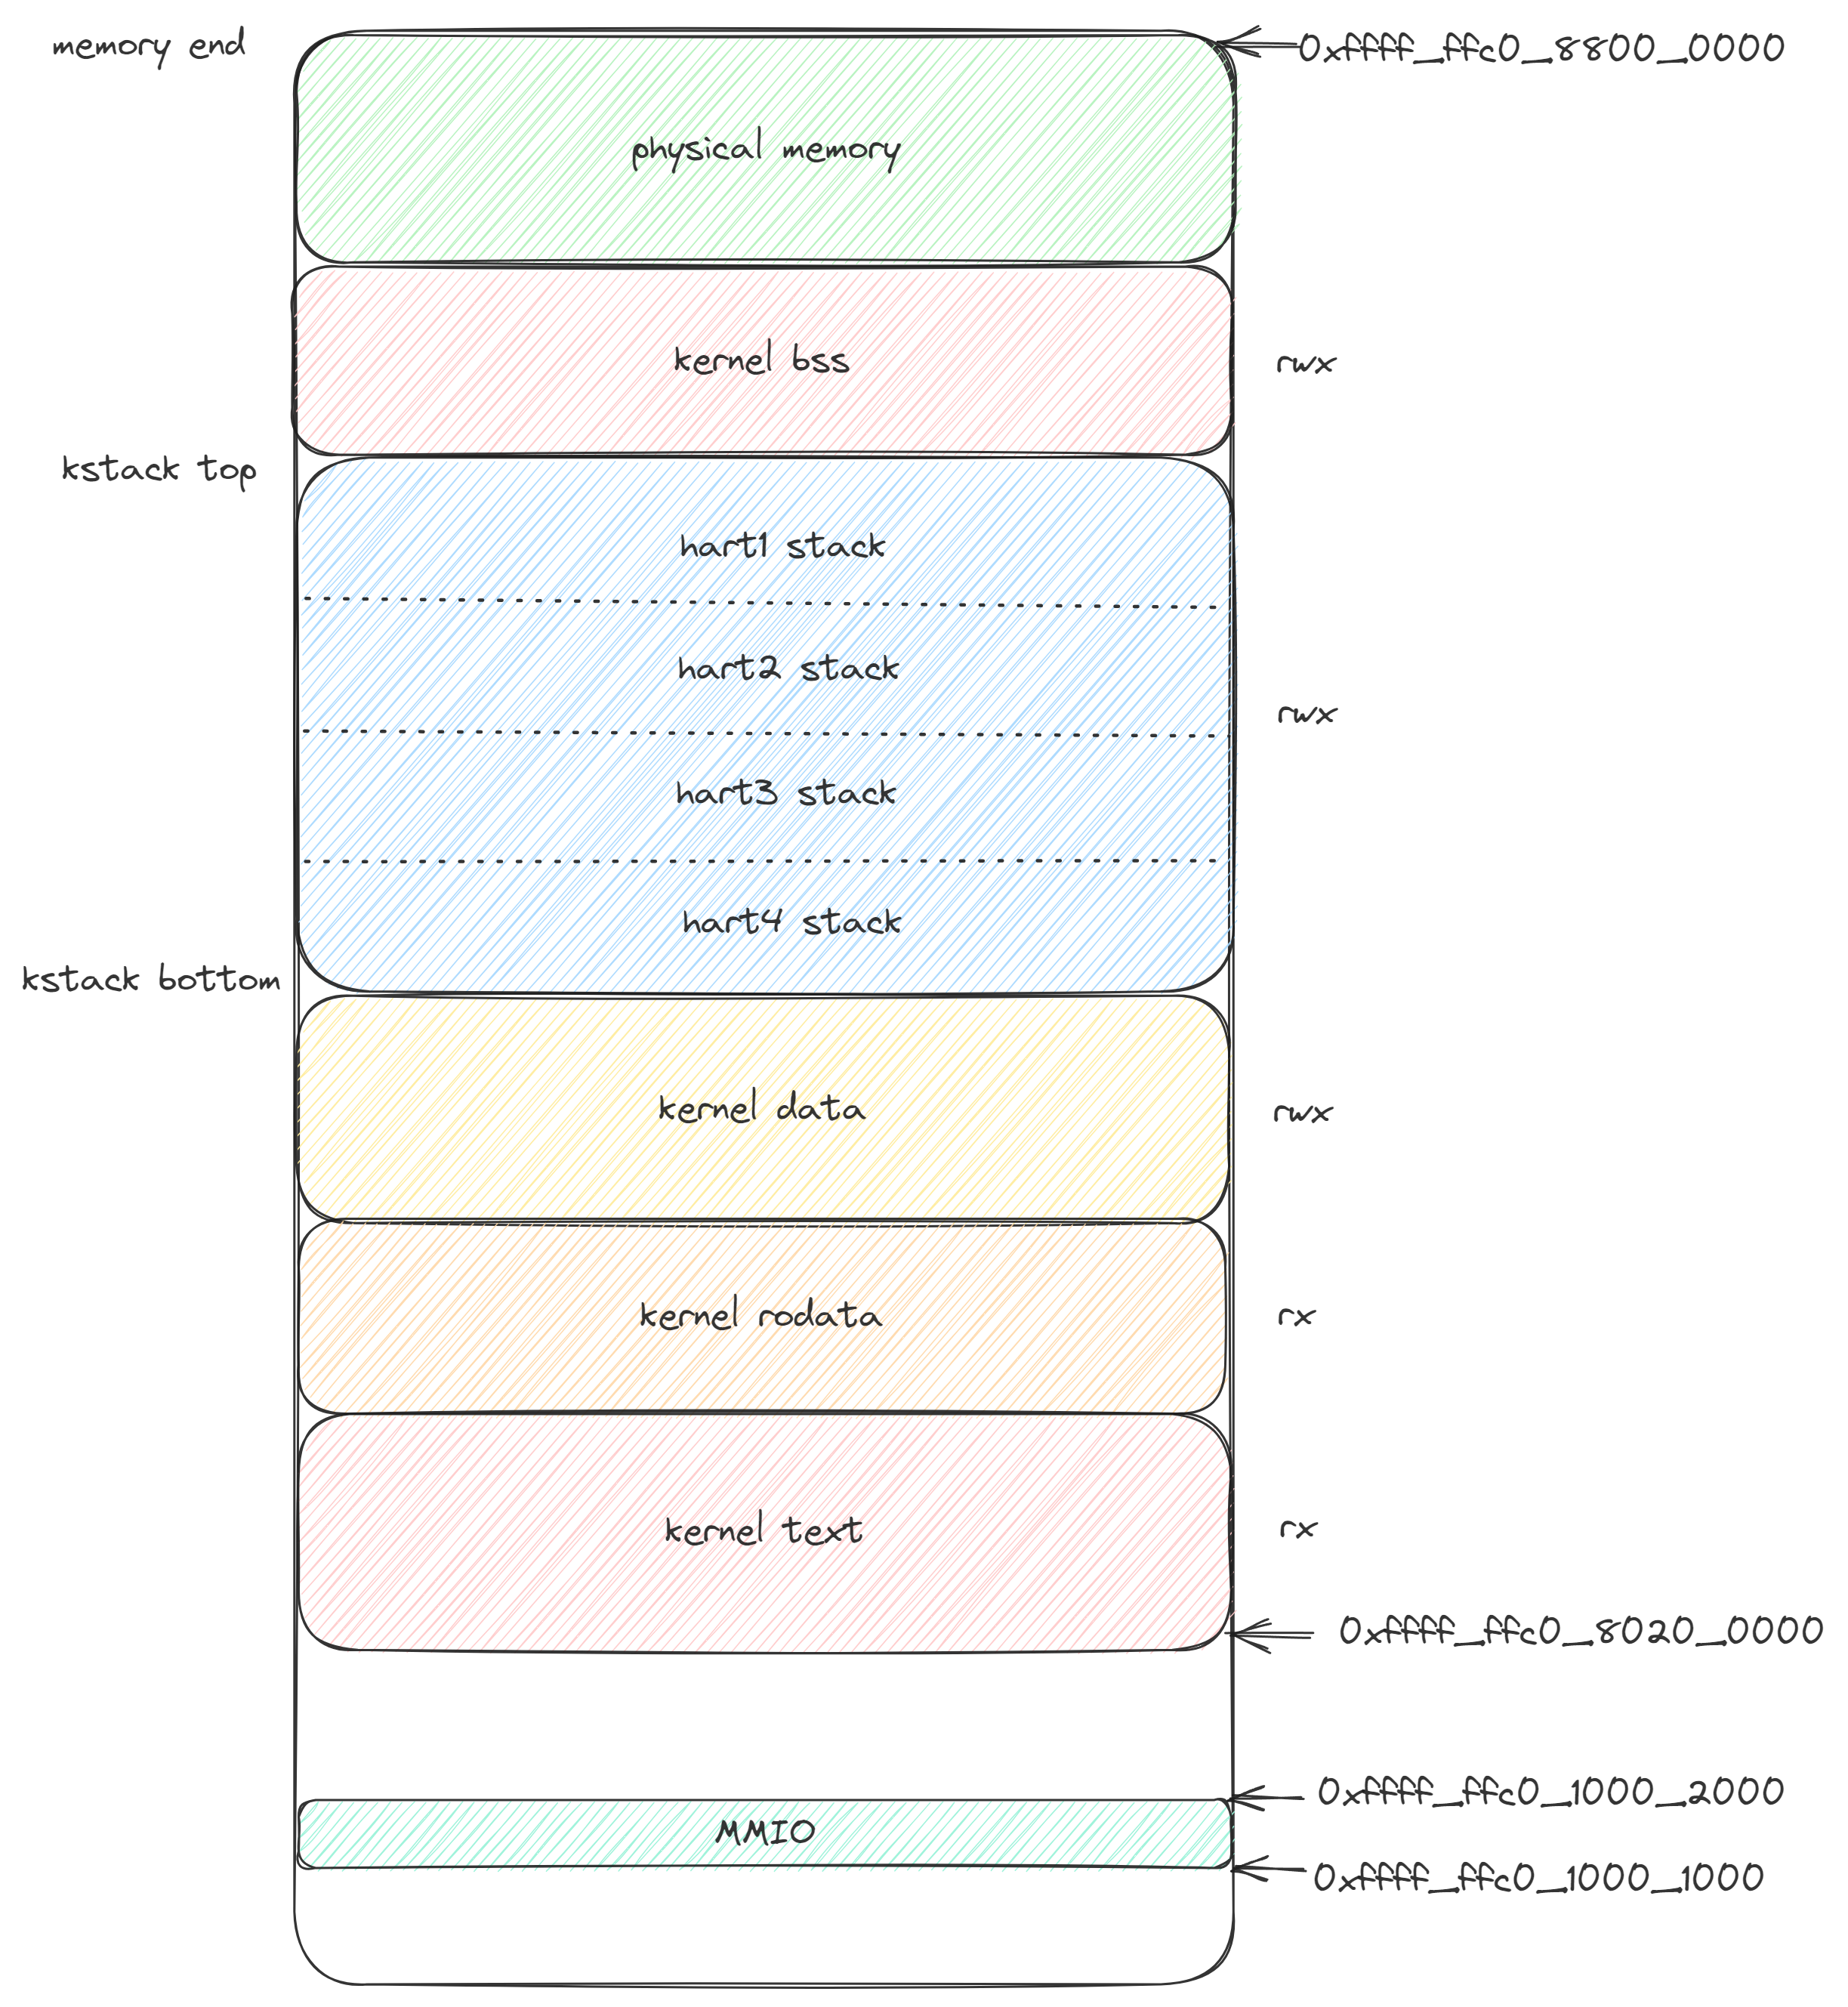
\includegraphics[width=.8\linewidth]{figure/kernel_mem.png}
    \caption{内核地址空间}
    \label{pic:kernel_mem}
\end{figure}

\paragraph{进入内核}~{}

那么如何在启动的时候快速映射到高位呢?我们难道要用汇编手写一个SV39三级页表?其实没必要,在RISC-V SV39里,MMU的翻译逻辑是逐级查找,一旦遇到页表项包含了V位,便停止查找,并不需要查满三层,这意味着我们可以直接映射一个巨页(即只用一级页表),手写一个根页表并不是一件非常复杂的事情,我们只需要将0x8000\_0000和0xffff\_ffc0\_8000\_0000这两个巨页添加到页表项即可,具体逻辑如下所示:
\begin{tcolorbox}[title=\textbf{os/src/entry.S}]
\begin{minted}[baselinestretch=1, fontsize=\small]{gas}
boot_pagetable:
    # we need 2 pte here
    # 0x0000_0000_8000_0000 -> 0x0000_0000_8000_0000
    # 0xffff_fc00_8000_0000 -> 0x0000_0000_8000_0000
    .quad 0
    .quad 0
    .quad (0x80000 << 10) | 0xcf # VRWXAD
    .zero 8 * 255
    .quad (0x80000 << 10) | 0xcf # VRWXAD
    .zero 8 * 253
\end{minted}
\end{tcolorbox}

另外,我们将内核的栈段划分为多段作为每个核心的内核栈,在进入内核的时候根据sbi传入的核心id计算出对应核心的内核栈的范围,并将其值赋给sp指针即可。

\paragraph{用户地址空间}~{}

用户地址空间见下\cref{pic:user_mem}所示,我们将文件映射及匿名映射的内存地址放置到用户地址空间的最高位,将堆段放置到栈段之上,其他的段都是在解析程序elf文件时映射的。

\begin{figure}[hbt]
    \centering
    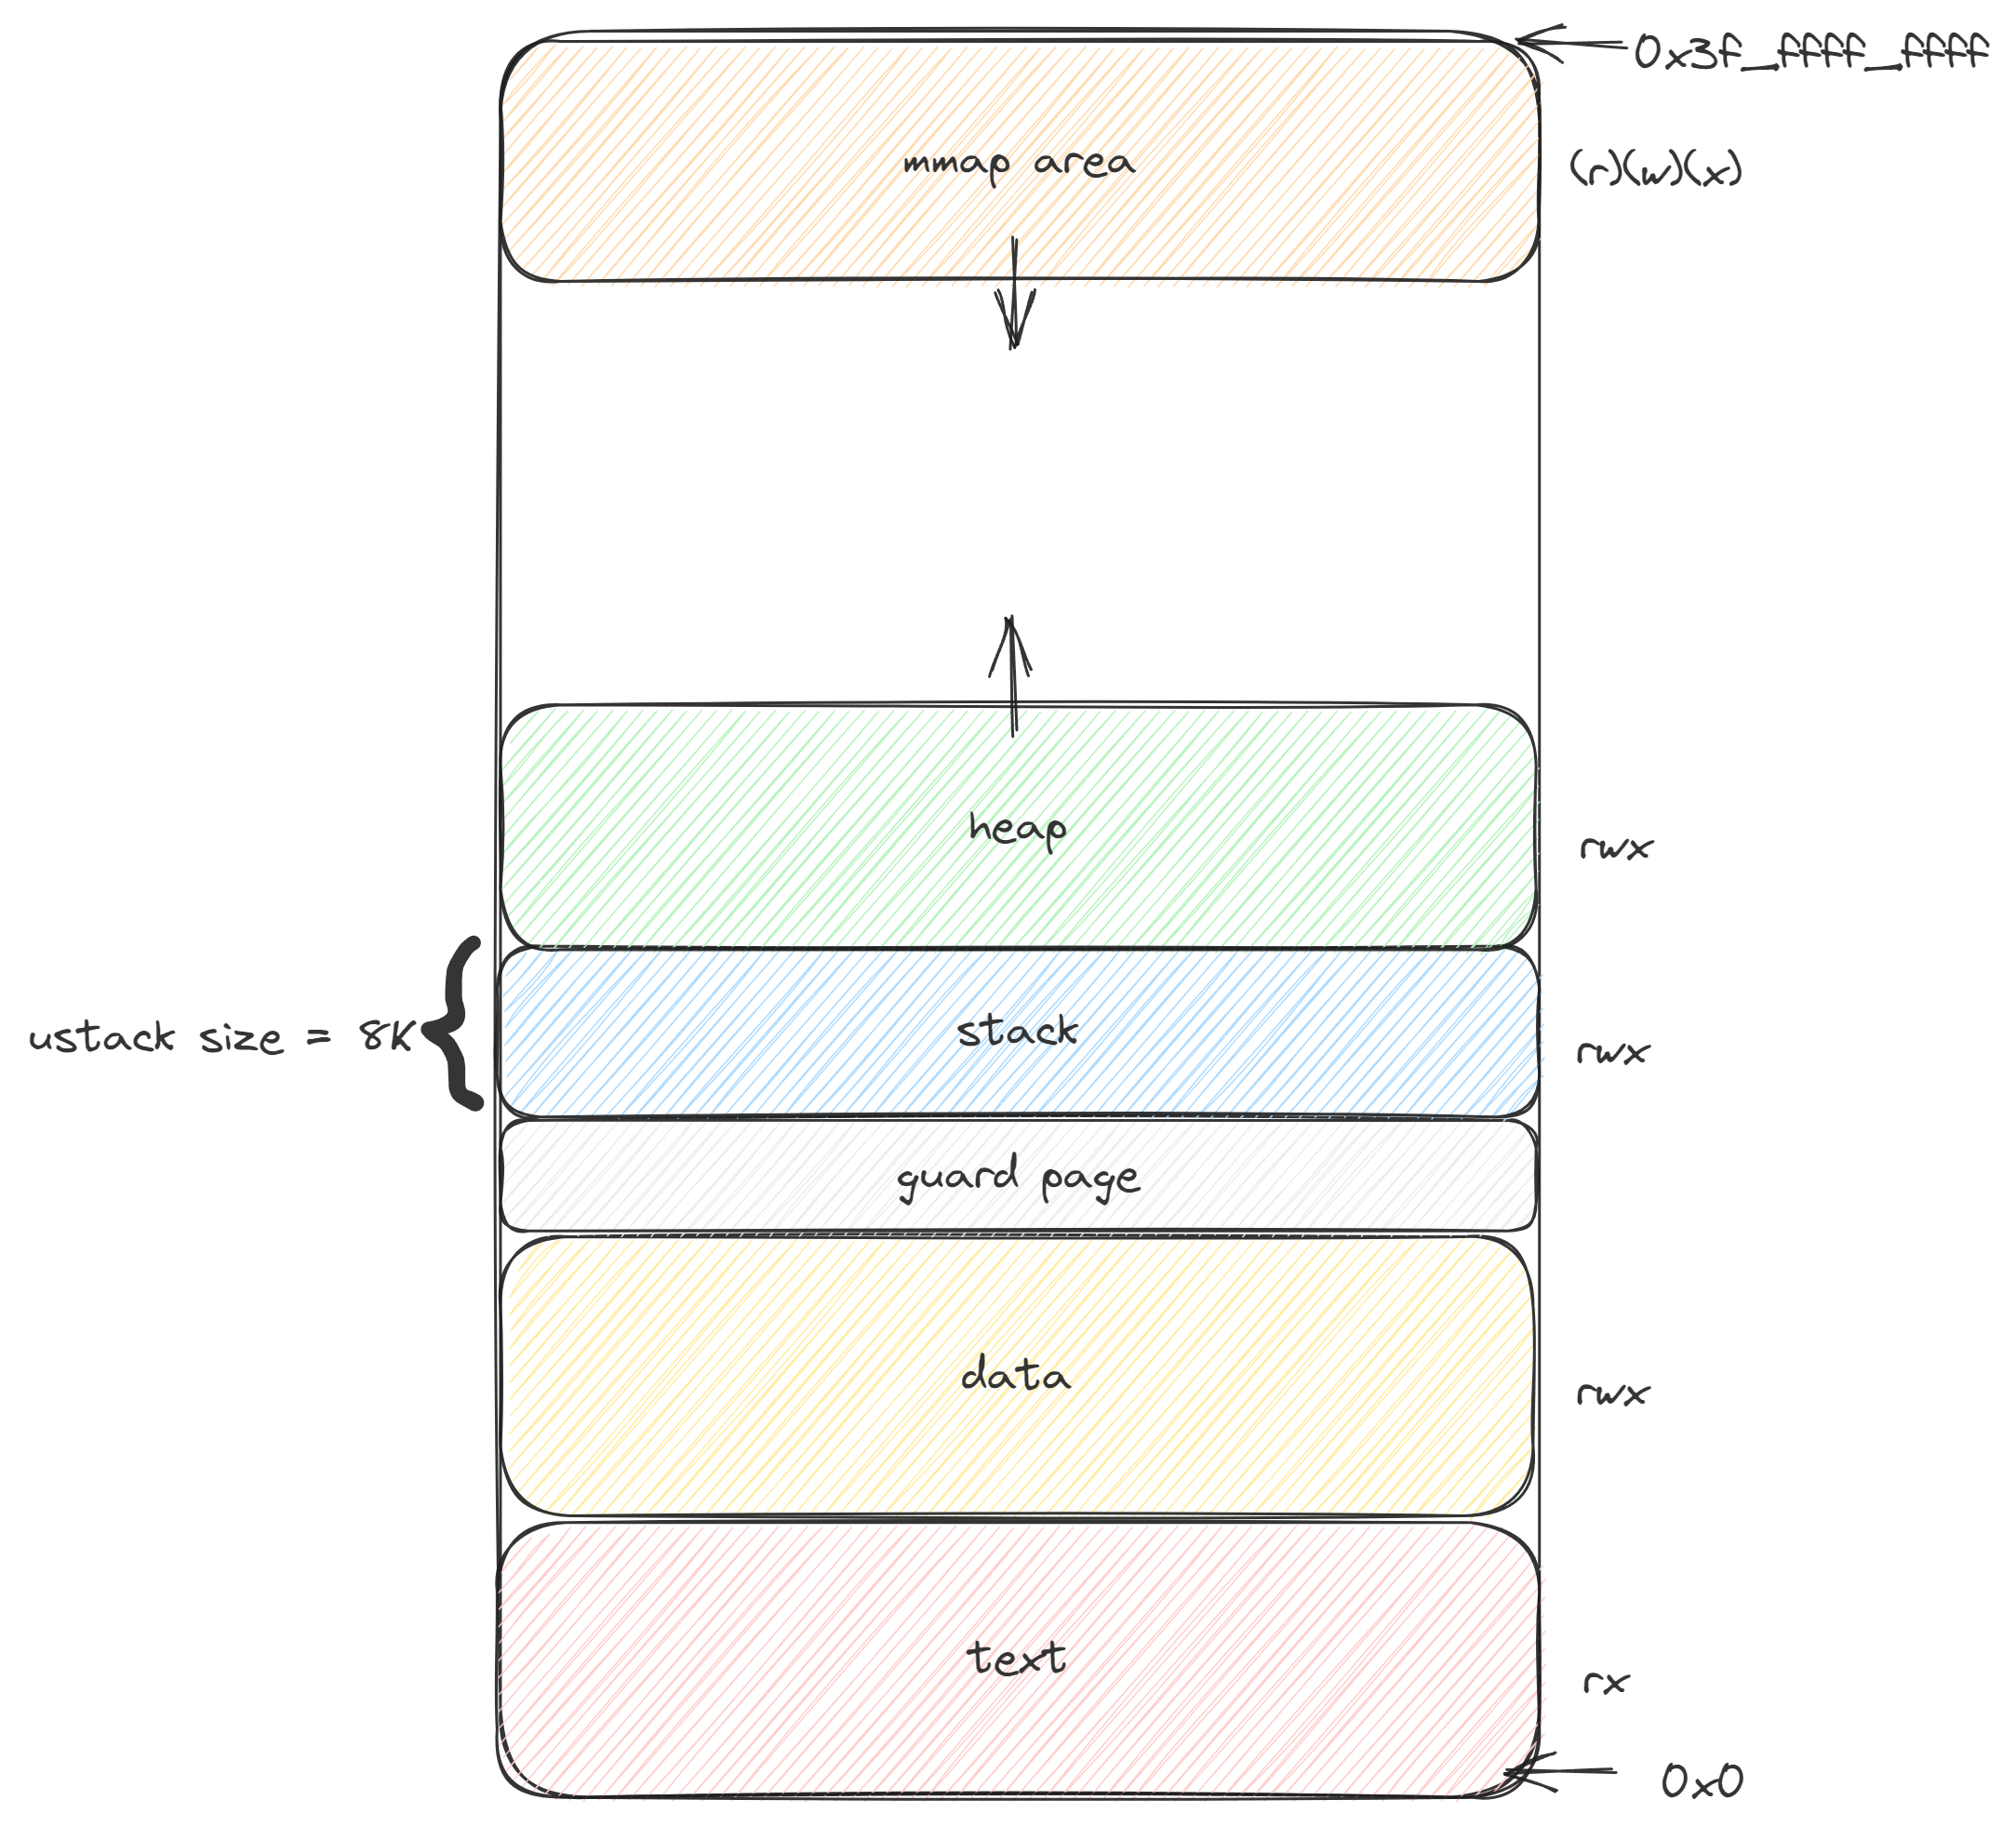
\includegraphics[width=.8\linewidth]{figure/user_mem.png}
    \caption{用户地址空间}
    \label{pic:user_mem}
\end{figure}

\subsubsection{内存映射}

\paragraph{内核空间内存映射}~{}

对于内核空间来说,所有的段都是直接映射,这里的直接映射指物理页地址加上一个偏移量(即0xffff\_ffc0),包括物理页帧,因此在将物理页帧分配给用户时需要将地址减去偏移量才能得到真正的物理地址。

\paragraph{用户空间内存映射}~{}

对于用户空间来说,所有的段都是物理页帧随机映射,我们在内核中维护一个物理页帧分配器用以管理所有的物理页帧,对于每个物理页帧,我们采用了Rust中的原子引用计数Arc来维护,当物理页帧的引用计数为0时自动释放,我们通过覆盖物理页帧的析构函数来实现将空闲物理页帧回收至物理页帧分配器,这是一种RAII的思想,广泛运用在我们的内核中,同时Arc也大大简化了后面我们实现写时复制的步骤。

\subsubsection{内存管理相关数据结构}
\begin{figure}[hbt]
    \centering
    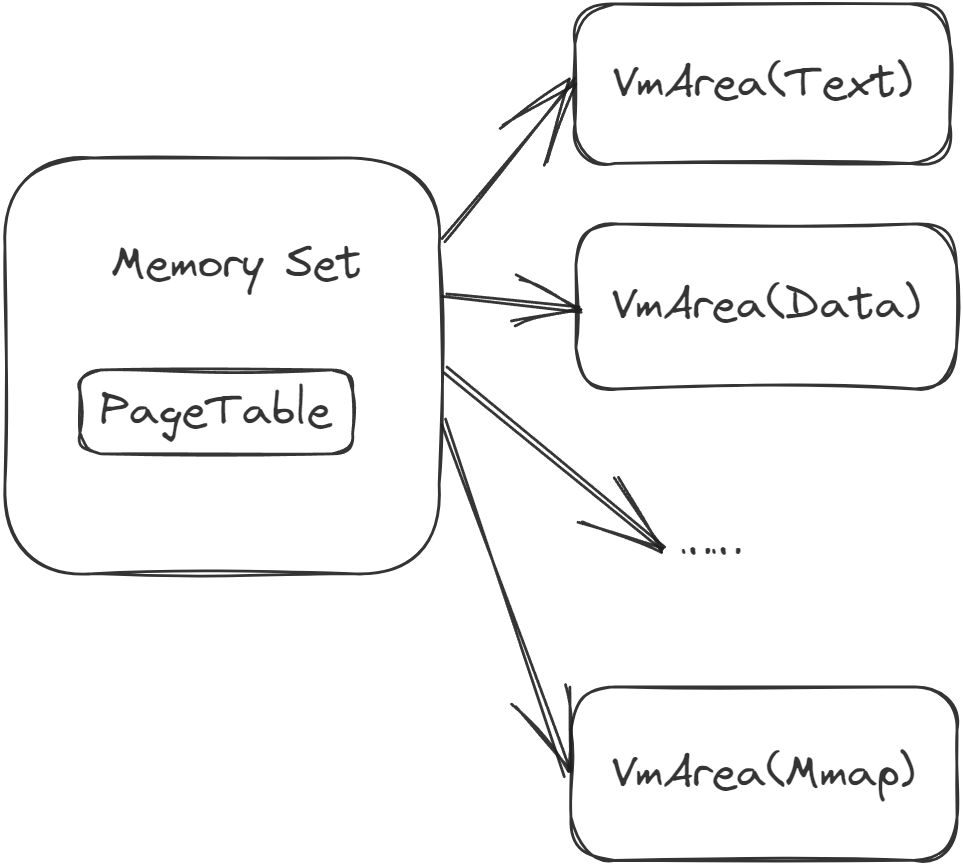
\includegraphics[width=.7\linewidth]{figure/mem_set.png}
    \caption{进程地址空间数据结构}
    \label{pic:mem_set}
\end{figure}

下面介绍内核中内存管理相关的重要数据结构。

\paragraph{MemorySet}~{}

\begin{tcolorbox}[title=\textbf{os/src/entry.S}]
\begin{minted}[baselinestretch=1, fontsize=\small]{rust}
/// memory set structure, controls virtual-memory space
pub struct MemorySet {
    /// we should ensure modifying page table exclusively(e.g. through process_inner's lock)
    /// TODO: optimization: decrease the lock granularity when handling page fault
    pub page_table: Arc<SyncUnsafeCell<PageTable>>,
    /// start vpn -> vm_area
    areas: BTreeMap<VirtPageNum, VmArea>,
    /// heap range
    pub heap_range: Option<HeapRange>,
}
\end{minted}
\end{tcolorbox}
如上所示,每个进程会有一个MemorySet成员表示其地址空间,该结构体包含一个页表,以及通过B树维护对各个内存段的索引,便于根据给定的虚拟地址快速查找、删除或修改其对应的内存段。

\paragraph{VmArea}~{}

\begin{tcolorbox}[title=\textbf{os/src/entry.S}]
\begin{minted}[baselinestretch=1, fontsize=\small]{rust}
/// map area structure, controls a contiguous piece of virtual memory
pub struct VmArea {
    /// Vpn range
    pub vpn_range: VPNRange,
    /// We don't need to use lock because we've locked the process
    /// inner every time we handle page fault
    pub data_frames: UnsafeCell<FrameManager>,
    /// Map type
    pub map_type: MapType,
    /// Map permission
    pub map_perm: MapPermission,
    /// Mmap flags
    pub mmap_flags: Option<MmapFlags>,
    /// Page fault handler that is invoked when page fault
    pub handler: Option<Box<dyn PageFaultHandler>>,
    /// Backup file(only used for mmap)
    pub backup_file: Option<BackupFile>,
}
\end{minted}
\end{tcolorbox}
如上所示,VmArea即代表某个内存段,各个成员的作用如注释所述,值得注意的是,VmArea有一个handler成员,当发生页错误时,我们可以根据发生页错误的地址查找出相应的VmArea,然后再调用其handler成员处理这个页错误,从而让页错误的维护工作变得统一且具有可扩展性。

\subsubsection{懒分配与写时复制}

为了提高性能,我们应当尽可能地减少拷贝和申请内存的次数,目前Titanix里采用了懒分配和写时复制的技术来减少开销。

\paragraph{懒分配}~{}

目前Titanix里的懒分配主要有以下三个方面:
\begin{enumerate}
    \item 用户栈的懒分配:在进程构建出来的时候,我们给用户进程划分一个虚拟地址栈空间但不实际分配物理地址,当用户访问栈空间时再通过缺页中断分配物理页。
    \item 用户堆的懒分配:类似与用户栈的懒分配,当用户调用brk系统调用增长进程空间时,我们只增长虚拟地址空间而不实际分配物理内存,当用户真正读写该堆空间时再通过缺页中断进行物理页分配。
    \item mmap内存段的懒读取:当用户进行mmap系统调用时,我们记录下对应的文件指针以及映射的偏移量范围但不进行实际读取,当用户真正读写到该内存段时再通过缺页中断读取相应文件的相应位置的内容。
\end{enumerate}

\paragraph{写时复制}~{}

当进行fork系统调用构造出新的进程时,我们不需要将父进程地址空间的全部内存拷贝一份,而是让子进程与父进程共享物理内存页,这样做的开销就只有修改页表了。注意到RISC-V中页表项的标志位中留了一个保留位,我们可以将其设置为COW位,在fork的时候需要将具有写权限的内存段的写标志位去掉,同时添上COW位。值得注意的是,在copy-on-write的时候我们还需要注意某个内存段是否是懒分配的内存段,若是,我们便不需要共享物理页,直接新增一个虚拟地址内存段即可。

另外,前文提到我们对物理页帧使用Arc(原子引用计数)进行维护,在这里派上了用场,因为在COW的时候父子进程会同时持有对同一物理页面的所有权,对于一个物理页面,我们需要等到其引用计数为0的时候才可以将其回收进空闲物理页帧中,这里直接利用了Arc的特性。

\paragraph{页错误处理函数}~{}

懒分配和写时复制在后面还需要进行扩展,如elf文件懒加载等,而这项技术的关键在于通过缺页中断进行真正的分配或者加载,因此我们需要设计一个可扩展的统一的页错误处理方式以便于后期的维护与扩展。通过参考Linux,我们为每个内存段(VmArea)设置一个页错误处理函数,利用Rust里的动态分发实现多态,从而可以使用统一的接口来存储页错误处理函数,该trait如下所示:
\begin{tcolorbox}[title=\textbf{os/src/mm/memory\_set/page\_fault\_handler.rs}]
\begin{minted}[baselinestretch=1, fontsize=\small]{rust}
/// General page fault handler
pub trait PageFaultHandler: Send + Sync {
    /// Handle the specific virtual page fault
    fn handle_page_fault(
        &self,
        va: VirtAddr,
        vma: &VmArea,
        page_table: &mut PageTable,
    ) -> GeneralRet<()>;

    ///
    fn is_legal(&self, _scause: Scause) -> bool {
        todo!();
    }

    /// Used for cloning in `fork`
    fn box_clone(&self) -> Box<dyn PageFaultHandler>;
}
\end{minted} 
\end{tcolorbox}

\subsubsection{用户地址检查}

在Titanix中,用户和内核共享地址空间,因此在访问用户态的内存时不需要同Xv6那样通过软件查询页表,而可以直接解引用访问。但直接解引用会带来一个问题,如果用户态传入的地址是一个不合法的地址,那在内核态直接解引用就会导致内核崩溃,因此对于用户态传入的地址,我们需要谨慎判断。我们采用这样一个方案,首先实现一个内核态异常的处理函数,当想要读写某个用户地址段时,先将修改中断向量的值为以下汇编函数的地址:
\begin{tcolorbox}[title=\textbf{os/src/mm/memory\_set/page\_fault\_handler.rs}]
\begin{minted}[baselinestretch=1, fontsize=\small]{rust}
// if pagefault occurs, return: (a0, a1) <- (1, scause).
    .align 6
__try_access_user_error_trap:
    csrw sepc, ra   # ra -> __try_x_user_u8's return addr
    li a0, 1
    csrr a1, scause
    sret
\end{minted} 
\end{tcolorbox}
以上函数即为

\subsubsection{多核启动}


\subsubsection{页缓存}
\subsection{文件系统}

\subsubsection{概述}

对于文件系统模块,我们的主要目标是使该模块结构合理清晰,实现简单,功能符合大赛要求,最主要的拥有良好的可扩展性。
目前 Titanix 的文件系统模块的总体已经完成还有一些细节和 BUG 需要完善。

\paragraph{虚拟文件系统}~{}

Titanix 的文件系统模块借鉴了 Linux 中 VFS(虚拟文件系统)的设计,使得
Titanix 可以支持多种文件系统我们对文件系统和文件分别定义了统一的接口,
open,write,read,mkdir 等系统调用的处理函数可以通过这些接口来对具体的文件系
统和文件进行操作,而不需要考虑各个文件系统的实现细节。如果需要让 Titanix 支
持新的文件系统,只需要为这个文件系统以及这个文件系统的文件实现统一的接
口即可。

文件系统和文件接口是以 trait 的方式定义的一共有两类抽象接口:

\begin{enumerate}
    \item 文件系统抽象接口:FileSystem trait,每一个文件系统都需要实现该 trait 该接口非常简单,主要的成员只有 root\_inode,通过该接口可以获得文件系统的根索引。
    \item 文件抽象接口:如果要实现File trait,必须先实现其依赖的父trait:Inode trait,而Inode trait要由要求实现InodeDevice,InodeDevice又要求注册的设备需要满足块设备或者字符设备的抽象,于是就有了虚拟文件系统的层级结构。
\end{enumerate}

\paragraph{FAT32文件系统}~{}

\subsubsection{虚拟文件系统}

VFS的功能是负责定义内核和文件系统之间的接口规范,因此我们在实现FAT32文件系统之前进行了VFS的设计与编写。同时希望我们的VFS具有一定的可扩展性,可以使得不同的文件系统在实现了VFS规定的接口之后即可与我们的Titanix进行对接,并迅速投入使用。此外,我们希望内核代码具有易读性以及良好的可维护性,于是我们在Linux的VFS基础之上,对其设计和相应的结构体进行了简化。为此我们进行了以下设计:

\paragraph{Inode \& Dentry}~{}

在FAT32文件系统当中没有inode,而一些文件系统当中又有一些特殊的结构体,为了简化设计,VFS当中只设计inode作为与下层实际文件系统相关联的结构体,并在inode基础之上抽象出文件类型(file),以及文件系统(filesystem);在file基础上抽象出默认文件(default file)、标准输入输出(stdio)、管道(pipe)和文件树(fd\_table),见下\cref{pic:vfs_layout}。

\begin{figure}[hbt]
    \centering
    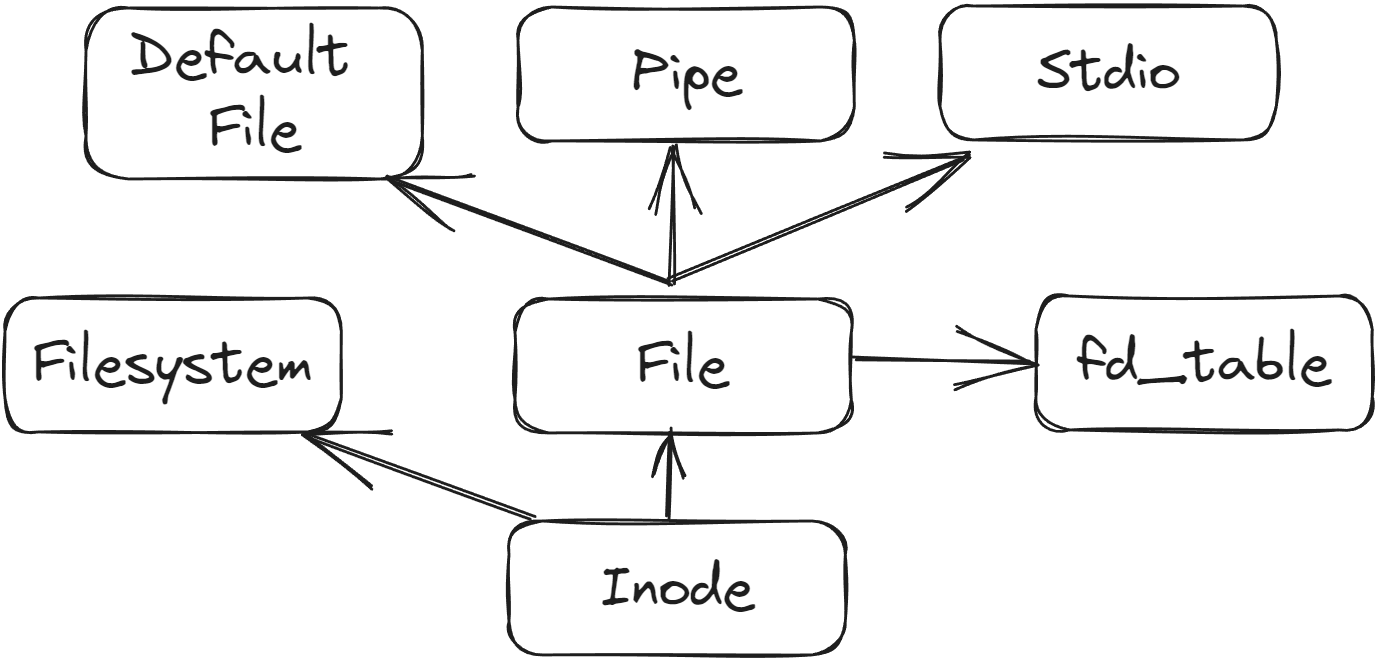
\includegraphics[width=.8\linewidth]{figure/vfs_layout.png}
    \caption{VFS框架}
    \label{pic:vfs_layout}
\end{figure}

对于Inode,由于Titanix中不存在dentry的概念,原本由dentry的负责的路径转实际inode的过程(lookup),现在应该交由inode负责。于是为了后续对inode内容的更改的便捷,我们设计了以下InodeMeta结构体:

% \newenvironment{codebox}[1]{
% \begin{tcolorbox}[title=\textbf{#1}]
% \begin{minted}{rust}
% }{
% \end{tcolorbox}
% }

% \begin{codebox}{xxxxstruct}
% pub struct jiwjjowjiwojofiew {
%     pub fuck: usize,
% }
% \end{minted}
% \end{codebox}


\begin{tcolorbox}[
title=\textbf{os/src/fs/inode.rs},
listing only,
breakable
]
\begin{minted}[breaklines, baselinestretch=1, fontsize=\small]{rust}
pub struct InodeMeta {
    /// inode number
    pub ino: usize,
    /// data address
    pub data: usize,
    /// type of inode
    pub mode: InodeMode,
    /// device id (only for block device and char device)
    pub rdev: Option<usize>,
    /// inode's device
    pub device: Option<InodeDevice>,
    /// path to this inode
    pub path: String,
    /// name which doesn't have slash
    pub name: String,
    /// a inode's unique id
    pub uid: usize,
    pub inner: Mutex<InodeMetaInner>,
}
\end{minted}
\end{tcolorbox}

并将可能需要更改的对象放在了IndoeMetaInner里面,这里给出InodeMetaInner结构体的设计:

\begin{tcolorbox}[
title=\textbf{os/src/fs/inode.rs},
listing only,
breakable
]
\begin{minted}[breaklines, baselinestretch=1, fontsize=\small]{rust}
pub struct InodeMetaInner {
    // pub offset: usize,
    /// inode' file's size
    pub size: usize,
    /// last access time, need to flush to disk.
    pub st_atim: TimeSpec,
    /// last modification time, need to flush to disk
    pub st_mtim: TimeSpec,
    /// last status change time, need to flush to disk
    pub st_ctim: TimeSpec,
    /// hash name(Note that this doesn't consider the parent uid)
    pub hash_name: HashName,
    /// parent
    pub parent: Option<Weak<dyn Inode>>,
    /// brother list
    pub brothers: BTreeMap<String, Weak<dyn Inode>>,
    /// children list
    pub children: BTreeMap<String, Arc<dyn Inode>>,
    /// page cache of the related file
    pub page_cache: Option<PageCache>,
    /// data len
    pub data_len: usize,
}
\end{minted}
\end{tcolorbox}

为什么要这样做呢?这是考虑到rust这门语言的特性。rust对于对象的可变性有着较高的要求,对于可变对象的可变引用,如果想要保证对象在并行线程之间的访问的安全性,需要使用智能指针来保证(我们使用Arc来将可能需要更改的对象包裹),但是智能指针(Arc)要求对象为不可变,这样的话,如果想要更改对象的值,我们只能通过unsafe块来包裹线程不安全的代码,并自己手动保证线程之间的访问安全。我们最开始是这样写的,但是后面发现这样会导致代码难以读懂,并且导致指针之间的关系复杂且曲折。实际上,这种写法是违背rust的特性的。rust这门语言希望你不要随意对Arc中的对象进行更改,如果一定需要,请``上锁"。那么有什么办法可以对某一对象在保持Arc的引用的同时还可以更改其中的某些一值?答案就是将这些可能需要更改的对象抽象出来,作为一个Inner对象,并在原来的对象中添加该Inner对象,但是需要用所来包裹保证更改时的线程安全,这样就有了我们的解决办法。

这样做还有另外一个好处,通过将可变对象和不可变对象分开,使得我们可以在访问可变对象的同时,只对Inner上锁,让外部的不可变对象的访问可以并行执行,极大的提高了访问的并行性。

\paragraph{Name Hash}~{}

由于文件系统的文件组织具有层次化的特点,往往都会存在父目录和子目录这样的关系,所以在Linux当中,对于文件查找,使用了哈希表的技术来加快文件名到对应的inode的查找。

Titanix效仿Linux,同样对inode和实际文件名(字符串类型)之间建立一层哈希映射,以便于快速地进行文件查找。为此我们设计了HashName结构体,该结构体完成了文件名(str类型)到u64类型的映射,当我们知道文件名之后,就可以调用该结构体实现的hash\_name方法进行哈希值的计算,并从构建的全局哈希表当中获取该inode的Arc引用。该结构体如下所示:

\begin{tcolorbox}[
title=\textbf{os/src/fs/hash\_name.rs},
listing only,
breakable
]
\begin{minted}[breaklines, baselinestretch=1, fontsize=\small]{rust}
#[derive(Clone, PartialEq)]
pub struct HashName {
    pub name_hash: u64,
    pub parent: usize,
    pub name: Arc<str>,
}
\end{minted}
\end{tcolorbox}

你可能注意到了,我们的HashName结构体中存在parent的字段,为什么要设置这个字段呢?这是因为文件系统的层次性让我们可以在文件查询的时候做一些``小手脚"。通常来将,我们查找文件是将以字符串标识的路径,转换成对应的inode,那么这个过程可以通过从根inode开始进行逐层查找,所以一般来讲,我们是通过父目录找到下一级的目录,然后逐级查找到对应的文件(inode),那么我们就可以使用父目录和子目录的名字来一起做哈希,这样可以使得我们的哈希能够铺得更加平,从而在查找的时候能够在更加小的范围内进行精确匹配,使得查找的速度加快。

为了实现该结构体的一些hash函数,我们参考了Github开源仓库rust-hash-table中对于哈希表的实现。核心方法hash\_name的实现如下:
\begin{tcolorbox}[
title=\textbf{os/src/fs/hash\_name.rs},
listing only,
breakable
]
\begin{minted}[breaklines, baselinestretch=1, fontsize=\small]{rust}
pub fn hash_name(parent: Option<usize>, name: &str) -> HashName {
    let parent_ptr = match parent {
        Some(p) => p as u64,
        None => 0 as u64,
    };
    HashName {
        name_hash: Self::myhash(parent_ptr, Self::str2num(name)),
        parent: parent_ptr as usize,
        name: Arc::from(name),
    }
}
\end{minted}
\end{tcolorbox}

\paragraph{Inode Cache}~{}

通过Name Hash来加速查找可以提高查找的速度,但是频繁的访问磁盘永远不是一个好的决定,于是Titanix采用了一贯的用于协调内外存访问速度不匹配问题的解决办法——开辟缓存!

我们通过设置全局对象INODE\_CACHE,来对可能会使用的inode进行缓存,由于需要保证线程之间的并行访问安全,我们需要对该对象上锁。对于INODE\_CACHE,他应该完成某一个文件的inode的文件名哈希值与inode自身的映射管理,于是我们在设计Titanix时,将INODE\_CACHE定义为以下形式:
\begin{tcolorbox}[
title=\textbf{os/src/fs/inode.rs},
listing only,
breakable
]
\begin{minted}[breaklines, baselinestretch=1, fontsize=\small]{rust}
lazy_static! {
    pub static ref INODE_CACHE: Mutex<HashTable<usize, Arc<dyn Inode>>> = Mutex::new(HashTable::new());
}
\end{minted}
\end{tcolorbox}
可以看见,我们在申明该全局对象时,采用了lazy allocation的方式以帮助我们更好得实现内存管理,这里使用了rust的lazy\_static模块。

\paragraph{路径解析}~{}

对于路径解析,Titanix效仿Linux实现inode的lookup查找,利用文件名哈希值来加速查找,并利用INODE\_CACHE来减少访问磁盘的次数,我们给出了以下lookup方法:
\begin{tcolorbox}[
title=\textbf{os/src/fs/inode.rs},
listing only,
breakable
]
\begin{minted}[breaklines, baselinestretch=1, fontsize=\small]{rust}
fn lookup(&self, this: Arc<dyn Inode>, name: &str) -> Option<Arc<dyn Inode>> {
    let key = HashName::hash_name(Some(self.metadata().uid), name).name_hash as usize;
    let value = INODE_CACHE.lock().get(&key).cloned();
    match value {
        Some(value) => Some(value.clone()),
        None => {
            debug!(
                "cannot find child dentry, name: {}, try to find in inode",
                name
            );
            let target_inode = self.try_find_and_insert_inode(this, name);
            match target_inode {
                Some(target_inode) => Some(target_inode.clone()),
                None => None,
            }
        }
    }
}
\end{minted}
\end{tcolorbox}
从该方法的参数可以看出,这是一个成员函数,如何调用该方法呢?需要一个inode对象通过``."的方式来访问该成员方法。从这里就可以看出我们的lookup的逻辑,实际上是父亲inode调用lookup函数查找对应的孩子inode的过程。从上面的代码不难看出,我们会先尝试在INDOE\_CAHCE当中查找是否存在对应的inode,然后如果不存在,才开始调用try\_find\_and\_insert\_inode函数,试图在实际文件系统当中查找该inode,但是如果查找失败,那么返回值为None,交由上层判断处理。

对于try\_find\_and\_insert\_inode函数,我们将其作为VFS与实际文件系统相衔接的部分,这一方法负责调用VFS提供给实际文件系统的一些接口来实现从实际文件系统中查找对应的inode,由于调用该方法往往意味着在内存的INODE\_CACHE当中没有找到该inode,所以该方法顺带将找到的inode添加到INODE\_CACHE当中。以下给出该方法的代码:
\begin{tcolorbox}[
title=\textbf{os/src/fs/inode.rs},
listing only,
breakable
]
\begin{minted}[breaklines, baselinestretch=1, fontsize=\small]{rust}
fn try_find_and_insert_inode(
        &self,
        this: Arc<dyn Inode>,
        child_name: &str,
    ) -> Option<Arc<dyn Inode>> {
    let key = HashName::hash_name(Some(self.metadata().uid), child_name).name_hash as usize;
    self.load_children(this);
    debug!(
        "children size {}",
        self.metadata().inner.lock().children.len()
    );
    let target_inode = self
        .metadata()
        .inner
        .lock()
        .children
        .get(child_name)
        .cloned();
    match target_inode {
        Some(target_inode) => {
            // find the inode which related to this subdentry
            INODE_CACHE.lock().insert(key, target_inode.clone());
            Some(target_inode.clone())
        }
        None => {
            debug!("Cannot find {} in children", child_name);
            None
        }
    }
}
\end{minted}
\end{tcolorbox}
这里面的load\_children方法就是提供给实际文件系统的接口,用于向内存当中载入给定inode的孩子inode。

在上面单层查找的基础之上,我们实现了从根inode开始查找的代码:
\begin{tcolorbox}[
title=\textbf{os/src/fs/inode.rs},
listing only,
breakable
]
\begin{minted}[breaklines, baselinestretch=1, fontsize=\small]{rust}
/// Look up from root(e.g. "/home/oscomp/workspace")
    pub fn lookup_from_root(
        // file_system: Arc<dyn FileSystem>,
        path: &str,
    ) -> Option<Arc<dyn Inode>> {
    let path_names = Path::path2vec(path);
    let root_fs = FILE_SYSTEM_MANAGER
        .fs_mgr
        .lock()
        .get("/")
        .cloned()
        .expect("No root fs is mounted");
    let mut parent = root_fs.metadata().root_inode.clone().unwrap();
    for name in path_names {
        match parent.lookup(parent.clone(), name) {
            Some(p) => parent = p,
            None => return None,
        }
    }
    Some(parent)
}
\end{minted}
\end{tcolorbox}
该方法并不是一个关联方法,而是一个静态方法。抽象出该方法的目的是为了编写内核系统调用时能够更加有逻辑,并将大量重复代码进行复用。

\paragraph{文件系统抽象}~{}

Titanix为所有的文件系统建立一层抽象,通过让实际文件系统实现该FileSystem trait来将自己接入Titanix。为了在mount的时候能够区分不同的文件系统类型,Titanix将自己支持的文件系统类型直接硬编码到了内核当中,我们设计了FileSystemType这个枚举类型:
\begin{tcolorbox}[
title=\textbf{os/src/fs/file\_system.rs},
listing only,
breakable
]
\begin{minted}[breaklines, baselinestretch=1, fontsize=\small]{rust}
#[derive(Clone)]
pub enum FileSystemType {
    VFAT,
    EXT2,
    NFS,
}
impl FileSystemType {
    pub fn fs_type(ftype: String) -> Option<Self> {
        match ftype {
            vfat => Some(Self::VFAT),
            ext2 => Some(Self::EXT2),
            nfs => Some(Self::NFS),
            _ => None,
        }
    }
    pub fn new_fs(&self) -> impl FileSystem {
        match self {
            Self::VFAT => {
                // let fs = FAT32FileSystem::new();
                let fs = TestFs::new();
                fs
            }
            _ => {
                todo!()
            }
        }
    }
}
\end{minted}
\end{tcolorbox}
目前Titanix只能支持FAT32文件系统,后续还会支持更多类型的文件系统。

所有的文件系统通过实现Titanix中的FileSystem中的方法,可以实现与内核的对接,我们为实际文件系统实现了默认的初始化方法,但是这个只针对FAT32文件系统,后续还需要进行修改。实际文件系统通过将write\_inode、sync\_fs等方法实现来完成Titanix需要的文件交互动作。

\subsubsection{FAT32文件系统}
\subsection{信号系统}
\subsection{同步系统}

\section{总结与展望}

\end{document}